% This chapter should describe what was actually produced: the programs which were written, the hardware which was
% built or the theory which was developed. Any design strategies that looked ahead to the testing stage might 
% profitably be referred to (the professional approach again).

% Descriptions of programs may include fragments of high-level code but large chunks of code are usually best left % to appendices or omitted altogether. Analogous advice applies to circuit diagrams.
% Draw attention to the parts of the work which are not your own. Making effective use of powerful tools and 
% pre-existing code is often laudable, and will count to your credit if properly reported.
% It should not be necessary to give a day-by-day account of the progress of the work but major milestones may 
% sometimes be highlighted with advantage.

% ~4500 words

\documentclass[final,dissertation.tex]{subfiles}
\begin{document}

\chapter{Implementation}

In this chapter, I will describe how I implemented my project, describing challenges faced along the way. The implementation consists of the following:

\begin{itemize}
	\item A library for creating and processing Sphinx packets
	\item A library for sending and receiving messages on the Loopix network
	\item A command-line chat client that broadcasts messages to all clients on the network
	\item A testing framework for starting a test network
\end{itemize}

As Loopix uses the Sphinx packet format, I have implemented my own Java library for Sphinx. As such, the project is split into two libraries, with the low-level cryptographic elements and packet format implemented in Sphinx, and the high-level network decisions such as path selection and routing implemented in Loopix. The Loopix library provides a basic event-driven API for sending and receiving messages.

\section{Sphinx Library}

The Sphinx library provides an API for creating and processing Sphinx packets as generated by the \verb|sphinxmix| Python package. Since there was little documentation for \verb|sphinxmix|, significant efforts were required to reverse engineer functionality. This effort was necessary to meet the project goal of binary compatibility with the existing Python Loopix implementation. \verb|sphinxmix|'s implementation deviates in several places when compared with the algorithm described in the Sphinx paper, and the paper does not specify every implementation detail.

\subsection{Sphinx Parameters}

The \verb|SphinxParams| class encapsulates all of the cryptography and the various parameters for a Sphinx packet, such as the security parameter (key size) $\kappa$, header size, body size, various hash functions, the LIONESS block cipher, and operations on an elliptic curve group. The security parameter in this implementation is defined to be $\kappa = 128\text{ bits}$. The header and body size are parameters that can be chosen to fit certain applications. By default, Loopix uses a header and body size of 1024 bytes each.

I used the BouncyCastle Java library for cryptographic primitives. These are used to implement the following functions:

\begin{itemize}
	\item $\pi$: Used to encrypt the payload. Implemented using LIONESS, with AES-128-CTR as the stream cipher and SHA-256 as the hash function.
	\item $\pi^{-1}$: Used to decrypt the payload. This is the inverse of $\pi$, which is the LIONESS decryption function.
	\item $\mu$: A Message Authentication Code (MAC). Implemented using HMAC-SHA256, truncated to be $\kappa$ long.
	\item $\rho$: Used to encrypt the header. Implemented using AES-128-CTR.
	\item \verb|deriveAesKeyFromSecret|: Used to derive the AES key for payload encryption from a secret elliptic curve key. Implemented using SHA-256, truncated to be $\kappa$ long.
	\item Various hash functions:
		\begin{itemize}
			\item $h_\pi$: Used to key $\pi$
			\item $h_\mu$: Used to key $\mu$
			\item $h_\rho$: Used to key $\rho$
			\item $h_\tau$: Used to identify previously seen group elements
			\item $h_b$: Used to compute blinding factors
		\end{itemize}
		These are implemented by encrypting a block of all zeroes using AES-128-CTR, with an initialisation vector unique to each function.\footnote{The \verb|sphinxmix| package deviates from the paper here as the paper describes using SHA-256 for these hash functions.} For example, the pseudocode for $h_\rho$ is given below:
		\begin{javacode}
public byte[] hrho(byte[] key) throws CryptoException {
    return AES_ENCRYPT(key, ZERO_BLOCK, iv="hrhohrhohrhohrho");
}
		\end{javacode}
\end{itemize}

Operations on an elliptic curve group such as exponentiation are encapsulated inside the \verb|GroupECC| class. The curve chosen is the National Institute of Standards and Technology \verb|P-224| curve. There are concerns that the NIST curves are backdoored by the NSA \cite{safecurves}. The coefficients of the curves are generated from an unexplained ``random'' seed value. As the seed values are unexplained, an attacker can freely generate curves until finding a curve vulnerable to a secret attack. Due to the need for binary compatibility with \verb|sphinxmix|, it is not possible to use a more secure and efficient curve such as \verb|Curve25519|.\footnote{\verb|sphinxmix| has recently been updated with a variant called Ultrix that uses \verb|Curve25519| and has better performance. However, Loopix has not been updated.} This design allows other implementations of cyclic groups to be used in place of the current implementation with ease. As such, modifying the library to use a new curve would be trivial.

\subsection{Packet Creation}

A Sphinx packet has two parts, the header and the body. The header contains information to process the packet correctly, and the body contains the encrypted payload. The packet has the following structure:

\begin{javacode}
public class SphinxPacket {
    public SphinxHeader header;
    public byte[] body;
}
\end{javacode}

\subsubsection{Sphinx Packet Header}

The header has the following structure:

\begin{javacode}
public class SphinxHeader {
    public ECPoint alpha;
    public byte[] beta;
    public byte[] gamma;
}
\end{javacode}

\begin{itemize}
	\item \verb|alpha|, $\alpha$ is an elliptic curve group element ($\alpha = g^b$) used to derive the per-hop shared secret required to authenticate and process the rest of \verb|SphinxHeader|. It is also used to decrypt a layer of the Sphinx body payload.
	\item \verb|beta|, $\beta$ is a list of per-hop routing commands and padding that is encrypted in a nested manner. Each layer contains routing commands that is defined and processed by a Sphinx node.
	\item \verb|gamma|, $\gamma$ is a HMAC-SHA256 message authentication code tag that covers \verb|alpha| and \verb|beta|.
\end{itemize}

Header creation is handled in the \verb|SphinxClient| class. Input is a sequence of $\nu$ mix nodes $\{n_0,..,n_{\nu-1}\}$ and their corresponding public keys $\{y_0,...,y_{\nu-1}\}$, and outputs a \verb|SphinxHeader| object and a list of per-hop shared secrets $\{s_0,...,s_{\nu-1}\}$. The function signature for \verb|createHeader| is given below.

\begin{javacode}
private static SphinxHeaderData createHeader(SphinxParams params,
    List<byte[]> path,
    List<ECPoint> keys,
    byte[] destination) throws CryptoException
\end{javacode}

Header creation first starts with the derivation of key material for each hop. This key material will be used to encrypt and authenticate the rest of the header, and the packet payload. 

Initially, a random initial blinding factor $b \in_R \mathbb{Z}^*_q$ is chosen. A sequence of $\nu$ tuples $(\alpha_0, s_0, b_0),...,(\alpha_{\nu-1}, s_{\nu-1}, b_{\nu-1})$ is computed as follows:

\begin{itemize}
	\setlength\itemsep{-0.4em}
	\item $\alpha_0 = g^b,\ s_0 = y_0^b,\ b_0 = h_b(s_0)*b$
	\item $\alpha_1 = g^{b_0},\ s_1 = y_1^{b_0},\ b_1 = h_b(s_1)*b_0$
	\item ...
\end{itemize}

Each tuple $(\alpha_n, s_n, b_n)$ is defined as:

\begin{itemize}
	\item $\alpha_n$ is the group element used in the Elliptic-curve Diffie-Hellman key exchange (ECDH) to generate a shared secret. $\alpha_n$ can also be viewed as a public key.
	%$\alpha_n$ is the exponentiation of the group generator $g$ with a blinding factor $b_{n-1}$. 
	
	\item $s_n$ is the shared secret for hop $n$. 
	%$s_n$ is the exponentiation of the hop's public key $x_n$ with the blinding factor $b_{n-1}$, that is $s_n = x^{b_{n-1}}_n$. 
	As the public key $y_n$ is of the form $g^{x_n}$, then $s_n = (g^{x_n})^{b_{n-1}} = g^{{x_n}{b_{n-1}}}$. The shared secret is then passed into a key derivation function to produce an AES encryption key. The key derivation is done by passing the binary representation of the shared secret into the SHA-256 hash function and truncating the output to the security parameter $\kappa$.
	
	\item $b_n$, the blinding factor to be used for the next hop. This is computed by passing $s_n$ into the hash function $h_b$.\footnote{The \verb|sphinxmix| package deviates from the paper here as the paper describes $b_n = h_b(\alpha_n, s_n)$, but the actual implementation ignores $\alpha_n$ and does $b_n = h_b(s_n)$.}
	The blinding factor allows both senders and mix nodes to compute $\alpha_{n+1}$ from the shared secrets. This is necessary to avoid transmitting every group element unaltered throughout the path, as this would lead to linkable messages.
\end{itemize}

At the end of this derivation process, a list of $(\alpha_n, s_n, b_n)$ tuples, each corresponding to a header for a hop in the path is generated. \verb|header.alpha| is set as $\alpha_0$.

The next step is to generate filler strings $\phi_i$ that serves as encrypted padding for $\beta$, the routing information block. This is done by repeatedly encrypting the padding block with each hop's shared secret. The filler strings are to ensure that the header block has a constant length as it is processed by nodes. This prevents mix nodes from learning their position in the message's path.

The routing commands $\beta$ and MAC $\gamma$ are generated next. Starting from the last hop, a sequence of headers $M_{\nu-1},M_{\nu-2},...,M_{0}$, where $M_i = (\alpha_i, \beta_i, \gamma_i)$ is computed as follows:

\begin{itemize}
	\setlength\itemsep{-0em}
	\item $\beta_{\nu-1} = \rho(h_\rho(s_{\nu-1}), \{{\text{destination-identifier}}\|\phi_{\nu-1}\})_{[0..\text{header size}]}$
	\item $\beta_{i} = \rho(h_\rho(s_{i}),  \{|n_{i+1}| \| n_{i+1} \| \gamma_{i+1} \| \beta_{i+1}\})_{[0..\text{header size}]}$ for $0 \le i < \nu - 1$
	\item $\gamma_i = \mu(h_\mu(s_{i}), \beta_i)$
\end{itemize}

$\beta_i$ consists of either the destination identifier and the encrypted padding $\phi_{\nu-1}$, or the next hop in the path $n_{i+1}$ prefixed with its length $|n_{i+1}|$, a MAC $\gamma_{i+1}$ and a encrypted routing command block $\beta_{i+1}$ to forward to the next node. $\beta_i$ is then truncated to the header size.

\verb|header.gamma| is set to $\gamma_0$, and \verb|header.beta| is set to $\beta_0$. The final header structure when $\nu = 4\text{ hops}$ is illustrated in Figure~\ref{fig:sphinx_header}. At the end of this process, a \verb|SphinxHeader| object with the necessary data $M_0$ and a list of per-hop shared secrets are created. The list of shared secrets will be later used for encrypting the payload.


\begin{figure}[h]
	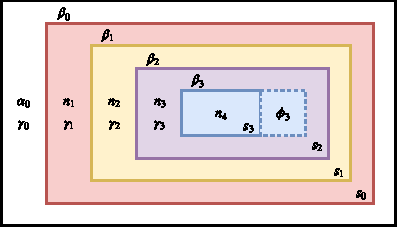
\includegraphics[width=\linewidth]{../figs/sphinx_header}
	\caption{Sphinx header for a packet with 4 hops}\label{fig:sphinx_header}
\end{figure}

\subsubsection{Sphinx Forward Packet Body}

Body creation is handled in the \verb|SphinxClient| class.  The function signature for creating an entire \verb|SphinxPacket| is given below.

\begin{javacode}
public static SphinxPacket createForwardMessage(SphinxParams params,
    List<byte[]> path,
    List<ECPoint> keys,
    Value destination,
    byte[] message) throws SphinxException
\end{javacode}

\verb|createForwardMessage| takes as inputs a sequence of mix nodes and their corresponding public keys as per the header generation section above, and a message $m$ of type \verb|byte[]|. It performs the following operations:

\begin{enumerate}
	\item \verb|message| is concatenated with the destination identifier and serialised using \verb|msgpack|, then padded to a fixed size.
	\item A call is made to \verb|createHeader| to generate a \verb|SphinxHeader| and the list of shared secrets $\{s_0,...,s_{\nu-1}\}$ to encrypt \verb|message| with.
	\item Starting from the terminal hop, \verb|message| is repeated encrypted using $\pi$ with a key derived from the hop's shared secret. That is,
		\begin{itemize}
			\setlength\itemsep{-0em}
			\item $\delta_{\nu-1} = \pi(h_\pi(s_{\nu-1}), m)$
			\item $\delta_i = \pi(h_\pi(s_{i}), \delta_{i+1})$
		\end{itemize}
	and as implemented:
	\begin{javacode}
byte[] delta = paddedBody;
for (int i = path.size() - 1; i >= 0; i--) {
    delta = params.pi(
        params.hpi(header.keys.get(i)), 
        delta
    );
}
	\end{javacode}
\end{enumerate}

The output of this process is the tuple $(M_0, \delta_0)$, which should be forwarded to the mix node $n_0$. The wire protocol for transmitting the tuple is determined by the consuming application. 

%\subsection{Packet Serialisation}
%
%msgpack, not actually used in Loopix

\subsection{Packet Processing}

The packet processing API is exported as the following:

\begin{javacode}
public class SphinxNode {
    public static SphinxProcessData processSphinxPacket(
        SphinxParams params, 
        BigInteger secret, 
        SphinxHeader header, byte[] delta)
        throws SphinxException, CryptoException
}
\end{javacode}

\begin{javacode}
public class SphinxProcessData {
	public byte[] tag;
	public byte[] routing;
	public SphinxHeader header;
	public byte[] delta;
}
\end{javacode}

The \verb|processSphinxPacket| function performs the majority of the per-hop packet processing. It handles authentication, decryption, and modifying the packet prior to forwarding it to the next node.

The mix node receives messages of the form $(M, \delta) = ((\alpha, \beta, \gamma), \delta)$. To decode the message, the mix node $n$, with private key $x_n$, performs the following steps:

\begin{enumerate}
	\item Calculate the hop's shared secret $s$ and replay tag $\tau$.
	\begin{itemize}
		\item $s = \alpha^{x_n}$
		\item $\tau = h_{\tau}(s)$
	\end{itemize}

	\item Derive the AES key required for further processing of the header and payload.
	\begin{javacode}
byte[] key = params.deriveAesKeyFromSecret(sharedSecret);
	\end{javacode}

	\item Validate the header by calculating the MAC and comparing the result with $\gamma$.
	\begin{javacode}
if (!Arrays.equals(header.gamma,
    params.mu(params.hmu(key), header.beta))) {
    throw new SphinxException("MAC mismatch.");
}
	\end{javacode}

	\item Pad $\beta$ with $2\kappa$ zero bytes such that the total length is the header size. This is done to keep the length of $\beta'$ which is forwarded to the next node the same. The padding is done before decryption to produce random-like padding after decryption.
	
	\item Decrypt $\beta$ using $\rho$.
	\begin{javacode}
byte[] B = params.rho(params.hrho(key), betaPadded);
	\end{javacode}

	\item Extract the routing command by using the length prefix from $\beta$. $\gamma'$ is also extracted from $\beta$. The rest of the $\beta$ is to be forwarded to the next hop as $\beta'$.
	
	\item Compute the blinding factor and thus the group element for the next hop.
		\begin{javacode}
BigInteger b = params.hb(key);
ECPoint alpha = group.expon(header.alpha, b);
		\end{javacode}
	
	\item The payload $\delta$ is decrypted. If this is the last hop, then this results in the decrypted message.
\end{enumerate}

At the end of this process, the tuple $(\tau, n, (\alpha', \beta', \gamma'), \delta')$ is produced. It is then up to the consuming application to check if it has seen $\tau$ before\footnote{In the original implementation of Loopix, there is a bug where the replay tag is not checked, losing some security in the process. }, parse the routing commands in $n$, and process the packet accordingly.

\subsection{Challenges Faced}

One of the goals was binary compatibility with the original Python implementation. As such, my implementation is based on the Python implementation. However, this introduced several challenges, mainly dealing with verbosity.

There are a lot of byte array manipulations, for example concatenation and slicing, which is easily done in Python as there are built-in operators. Another Python feature that is heavily used by \verb|sphinxmix| is the ease of encoding strings as byte arrays. For example, the following code computes the first encryption round of the LIONESS cipher in Python:

\begin{pythoncode}
k1 = self.hash(message[self.k:]+key+b'1')[:self.k]
c = self.aes_ctr(key, message[:self.k], iv = k1)
r1 = c + message[self.k:]
\end{pythoncode}
whereas in Java:
\begin{javacode}
byte[] k1 = Arrays.copyOf(
    hash(
        Arrays.concatenate(
            Arrays.copyOfRange(message, this.k, message.length), 
            key, 
            "1".getBytes(Charset.forName("UTF-8")))), 
        this.k);
byte[] c = aesEncrypt(key, Arrays.copyOf(message, this.k), k1);
byte[] r1 = Arrays.concatenate(c, 
    Arrays.copyOfRange(message, this.k, message.length));
\end{javacode}

Sphinx also makes use of \verb|msgpack| for serialising data. The Python API allows for simple serialisation of tuple data structures and dynamic objects which are widely used in \verb|sphinxmix|. However, the Java API is harder to use for such data structures. For example, the following is a function that is used to encode mix node information in Python:

\begin{pythoncode}
def encodeNode(idnum):
    return encode((Relay_flag, idnum))
\end{pythoncode}
and the same in Java:
\begin{javacode}
public static byte[] encodeNode(int idnum) throws IOException {
    Packer packer = Packer.getPacker();
    packer.packValue(new ImmutableArrayValueImpl(new Value[] {
        new ImmutableBinaryValueImpl(new byte[]{RELAY_FLAG}),
        new ImmutableLongValueImpl(idnum)
    }));
    return packer.toByteArray();
}
\end{javacode}

The Python implementation also lacked documentation, which hampered efforts in understanding the implementation details. Python's dynamic types meant that it was not clear at first glance what kind of arguments were being passed around. It also used OpenSSL libraries under the hood, which has a very different API compared to BouncyCastle or the Java Cryptography Architecture. For example, the cryptographic library \verb|sphinxmix| uses is \verb|petlib|, which simply defined the curve used with \verb|nid=713|. It was not immediately obvious which curve is used, and required finding the OpenSSL \verb|nid.h| header file to map the unique ID into a curve.

\section{Loopix Client Library}

The Loopix client library provides APIs for sending and receiving messages. It is a thin wrapper around the Sphinx packet format. It provides the public key infrastructure, handles path selection, extends Sphinx to support delayed forwarding, and handles protocol details such as sending cover traffic. Extensive understanding of the \verb|loopix| Python package was required since binary compatibility was a goal.

\subsection{Exported Interface}

The library exposes a \verb|LoopixClient| class that handles message sending and receiving. A \verb|LoopixClient| can be created from files generated by the Python implementation. This was done to simplify configuration management between the Java and Python nodes. Combined with the Docker-based architecture, it is possible to easily switch between the two. The configuration files contain the following parameters:

\begin{itemize}
	\setlength\itemsep{0em}
	\item \verb|EXP_PARAMS_PAYLOAD|, \verb|EXP_PARAMS_DROP|, \verb|EXP_PARAMS_LOOPS|, \verb|EXP_PARAMS_DELAY|: Scale parameters $\beta$ for the exponential distributions for message delays and message send rates. $\beta$ is the inverse of the widely used rate parameter $\lambda = 1/\beta$. Defined in terms of seconds.
	\item \verb|PATH_LENGTH|: Number of mix nodes to select for a path. 3 is used.
	\item \verb|DATABASE_NAME|: Path to the database containing information for nodes on the network.
	\item \verb|TIME_PULL|: Time each message retrieval poll from the provider.
	\item \verb|MAX_RETRIEVE|: Number of messages to return to client each poll.
	\item Client parameters such as the client's ID, provider ID, public key, and private key.
\end{itemize} 

\begin{javacode}
public class LoopixClient {
    public LoopixClient(String name, String host, short port, 
        String providerName, ECPoint publicKey, BigInteger privateKey, 
        Config config)
    public static LoopixClient fromFile(String configPath, 
        String publicPath, String privatePath);
    public void run();
    public void setMessageListener(LoopixMessageListener listener);
    public void addMessageToQueue(String clientName, byte[] data);
    public void setMessageBuilder(LoopixMessageBuilder builder)
}
\end{javacode}

\verb|LoopixClient| also exposes \verb|setMessageListener| for applications to process incoming messages. As Loopix provides sender anonymity, only the message is available.

\begin{javacode}
public interface LoopixMessageListener {
	void onMessageReceived(LoopixClient client, byte[] message);
}
\end{javacode}

\verb|LoopixClient| exposes two methods for sending messages. \verb|addMessageToQueue| adds a message to the send queue. \verb|setMessageBuilder| allows applications to be asked for a message whenever a real message needs to be sent. This allows applications to perform optimisations such as batching multiple messages intended for a single destination into a single packet, reducing the number of packets needed. This is used by the latency measurement tool described later in the paper to accurately measure processing overheads without including the time a message sits in the queue.

\begin{javacode}
public interface LoopixMessageBuilder {
	boolean isEmpty();
	ClientMessage getMessage();
}
\end{javacode}

\subsection{Public Key Infrastructure}

Sphinx, and by extension Loopix requires public key infrastructure to distribute knowledge of network nodes, such as their IDs, IP address, port number and public keys in order to route packets. This is achieved by distributing an SQLite database that is populated with information on every node that will be on the network. The SQLite database is also used in the Python implementation, allowing for reuse of existing code to generate the database. The database contains data of the following forms:

\begin{javacode}
public class LoopixNode {
    public String host;
    public short port;
    public String name;
    public ECPoint publicKey;
}
public class MixNode extends LoopixNode {
	public int groupID;
}
public class User extends LoopixNode {
    public String providerName;
}
public class Provider extends LoopixNode { }
\end{javacode}

Each node has the following fields: a network location in the form of \verb|<host>:<port>|, a \verb|name| that uniquely identifies the node, and an elliptic curve \verb|publicKey|. A mix node has an additional \verb|groupID| which indicates the layer of the network topology it is located in. A user has an additional \verb|providerName| that identifies the user's provider. The term \verb|User| is used instead of \verb|Client| to prevent confusion with the \verb|LoopixClient| class.

Preferably, the hostname would be replaced with an IP address. This would avoid any possible impact to anonymity due to the use of DNS. However, for a test network, the ability to use hostnames simplifies configuration. The database can be populated with hostnames that are resolved at run time, instead of having to statically allocate the IP addresses of every node in advance.

%It is not strictly necessary for the database to contain a user's network location, and is detrimental to both security and usability of the network. Only the provider needs to know the user's network location, and as part of the Loopix network protocol the user will register with the provider. This allows the provider to discover the user's network location. The current scheme would expose a user's network location, and allow adversaries to track a user moving from network to network. There is the additional issue of NAT traversal not preserving port numbers, as users behind a NAT is unable to receive packets without first establishing a connection to the provider, but the public port may differ from the private source port.

The \verb|ECPoint| data type is encoded using the scheme described in Section~\ref{sec:serialisation} and stored as a binary blob in the database.

Reading from the database is done using the \verb|sqlite-jdbc| library and the corresponding Java Database Connectivity (JDBC)
API built into Java. On start, the library will read and cache information on all mix nodes and the user's provider in memory to speed up lookups for path selection. SQL queries are used to lookup destination users and their provider. Optimally information on all users and providers are cached in memory as well, but this fails to scale as the number of users and providers are expected to be much larger than the number of mix nodes.

%\subsection{Path Selection}
%
%random selection, delay sampling

\subsection{Loopix Protocol}

This section describes the Loopix protocol. This includes packet formats, path selection and cover traffic details.

\subsubsection{Packet Format}

Loopix mainly uses the Sphinx packet format as described earlier, to provide end-to-end encryption and prevent intermediate nodes from learning additional information other than some routing details. However, there are control commands that do not use Sphinx, which may be considered bugs in the original implementation, as these packets reveal information that can break the Loopix security model. These have been maintained for backwards compatibility, but it could be easily fixed.

Loopix extends Sphinx by introducing its own routing commands. A routing command in Loopix contains the next hop's ID, hostname, port number, the number of seconds to delay forwarding the message, and a drop flag. The drop flag tells the processing node to drop the packet.

Loopix messages should be indistinguishable from each other. Loopix has the following types of Sphinx messages: 

\begin{itemize}
	\item \textbf{Real messages}
	\item \textbf{Loop cover messages} Sent to ourselves with the magic number \verb|HT| in the payload.
	\item \textbf{Drop cover messages} Sent to a random user with the drop flag set in the routing command for the provider and a random payload.
	\item \textbf{Dummy messages} Sent by providers to clients in response to a \verb|PULL| command, with the magic number \verb|HD| in the payload. In the original implementation, this is not a Sphinx packet but rather an unencrypted packet similar to the \verb|PULL| and \verb|SUBSCRIBE| commands. This modification was made to match behaviour described in the Loopix paper. Without the modifications, it is possible to distinguish dummy messages from real and loop cover messages when a client retrieves them from the provider, and analysis of bandwidth usage would be flawed. Although modifications were made to the Python implementation to support this, my implementation is still compatible with the original implementation.
\end{itemize}

Having magic numbers in the payload is not ideal, as having a type flag that is visible only to the destination node would be simpler. However, as the goal is compatibility with the Python implementation, this is not implemented.

Creation and processing of these messages are handled by the \verb|ClientCore| class, which abstracts away the details above and exposes functions such as \verb|createRealMessage|, \verb|createDropMessage|, \verb|createLoopMessage|, and \verb|processPacket|.  \verb|ClientCore| is initialised with a \verb|SphinxPacker| object that interacts with the Sphinx library to create packets. This design decision was made to reuse as much code as possible if I wanted to implement provider and mix node functionality. \verb|SphinxPacker| exposes a generic \verb|makePacket| function that is used to create any packet and handles encoding the various routing commands. As such, it also samples the delays for each hop from an $\text{Exp}(\mu)$ distribution, where $\mu$ is the inverse of the config parameter \verb|EXP_PARAMS_DELAY| such that $\mu = 1/\beta_\text{EXP\_PARAMS\_DELAY}$. Sampling from an exponential distribution is implemented by sampling from a uniform distribution $U \sim U(0,1)$ and using inverse transform sampling $X = -\ln(U)/\lambda = -\beta\ln(U)$:

\begin{javacode}
public static double randomExponential(double scale) {
    return Math.log(random.nextDouble())*(-scale);
}
\end{javacode}

There are two control commands that clients can send to providers:

\begin{itemize}
	\item \verb|SUBSCRIBE| messages. These are tuples of the form \verb|[|\verb|"SUBSCRIBE",| \verb|name,| \verb|hostName,| \verb|port,| \verb|publicKey|\verb|]|. A provider will begin storing messages for this client in an inbox.
	\item \verb|PULL| messages. These are tuples of the form \verb|["PULL", name]|. A provider will send \verb|MAX_RETRIEVE| messages back to the client, filling with dummy messages if there are less than \verb|MAX_RETRIEVE| messages in the client's inbox.
\end{itemize}

\subsubsection{Packet Serialisation} \label{sec:serialisation}

Sphinx requires Loopix to handle transmitting the Sphinx packet header and body to the next node. The approach taken by Loopix for serialising the packet is to encode the header and body using \verb|msgpack|. That is, the tuple \verb|(header, body) = ((alpha, beta, gamma), body)| is passed straight into \verb|msgpack|. Loopix also uses \verb|msgpack| for serialising the \verb|SUBSCRIBE| and \verb|PULL| control messages.

However, \verb|msgpack| does not natively support packing the \verb|ECPoint| type. This is done through the use of extension values in \verb|msgpack|, which hold a type ID and a byte array payload. \verb|ECPoint| is assigned type \verb|0x02|, and the payload is encoded as per RFC5480 \cite{RFC5480} using compressed ASN.1 encoding. The encoding is provided by BouncyCastle using \verb|ECPoint.getEncoded()| and \verb|ECCurve.decodePoint(byte[])| was used in the Java implementation.

\subsubsection{Networking}

Network communication in Loopix is done via UDP. The Apache MINA networking library was used to send and receive UDP packets. This was easier to use than Java's built-in \verb|DatagramSocket|. 

Upon starting the client, the client opens a UDP socket and listens for packets on a port listed in the public key infrastructure. The same socket is also used for sending packets. The only node that should be sending the client packets is the client's provider. Ideally, this means any packet from an unknown node is dropped. However, this is not implemented for two reasons: UDP spoofing can be used to bypass the check as there is no authentication between provider and client, and the use of hostnames instead of IP addresses complicates the check.

A scheduler using Java's built-in \verb|ScheduledExecutorService| is started. The scheduler is used for scheduling four events:

\begin{itemize}
	\item Sending real messages
	\item Sending loop cover messages
	\item Sending drop cover messages
	\item Sending provider pull requests
\end{itemize}

Sending provider pull requests is scheduled using the \verb|scheduleAtFixedRate| function, running \verb|retrieveMessages| every \verb|TIME_PULL| seconds. \verb|retrieveMessages| sends a \verb|SUBSCRIBE| and \verb|PULL| command to the provider.

\textbf{Path selection.} Messages are routed through 5 intermediate mix nodes, including providers. The path is: sender $\rightarrow$ ingress provider $\rightarrow$ layer 1 mix node $\rightarrow$ layer 2 mix node $\rightarrow$ layer 3 mix node $\rightarrow$ egress provider $\rightarrow$ recipient. Each mix node in the path is selected randomly. The recipient may be omitted for drop messages.

\textbf{Sending messages.} \verb|sendRealMessage| is periodically called by the scheduler. It checks two sources of messages: an attached \verb|LoopixMessageBuilder| and the send buffer. If there is a message, it will either ask for a message, or pop it from the buffer queue and sent. Otherwise, a drop message is generated and sent instead. This is shown in Figure~\ref{fig:loopix_network} as the blue lines. Each time \verb|sendRealMessage| is called, it samples a delay from an exponential distribution with parameter $1/\beta_\text{EXP\_PARAMS\_PAYLOAD}$, and the next call is delayed by the sampled value. This will cause a stream of messages to be emitted following the Poisson process $\text{Pois}(1/\beta_\text{EXP\_PARAMS\_PAYLOAD})$.

\textbf{Cover traffic.} The two cover traffic events occur similarly to the real message event. \verb|sendLoopMessage| sends loop messages, which are messages that have their recipients specified as the sender. Loop messages are emitted following the Poisson process $\text{Pois}(1/\beta_\text{EXP\_PARAMS\_LOOP})$. \verb|sendDropmessage| sends drop messages, which are messages with a random destination provider with a drop flag set such that the provider drops the packet instead of forwarding it. Drop messages are emitted following the Poisson process $\text{Pois}(1/\beta_\text{EXP\_PARAMS\_DROP})$. These are represented in Figure~\ref{fig:loopix_network} by the red and green lines.

\textbf{Processing messages.} In response to a \verb|PULL| request, a provider forwards messages held for a client, padding with dummy messages if necessary. The client first decodes and checks that the received packet has the correct \verb|msgpack| format that is expected. The Sphinx library is used to process the decoded packet, which returns a \verb|(header, body)| tuple. The client checks that the message is the final destination packet, and verifies that the destination is the client. Further processing is done to discard loop and dummy messages based on magic numbers in the payload. If it is a real message, then \verb|LoopixClient| calls the attached \verb|LoopixMessageListener| with the real payload.

\subsubsection{Challenges Faced}

Concurrency in the library introduced race conditions in the Sphinx library, as thread safety was never considered in the design phase and thus the library was not designed for concurrent operations. The client shared a single instance of the \verb|SphinxParams| object, which used a single instance of the AES \verb|Cipher| object. There are two operations that may run concurrently: receiving and sending messages. This may result in corrupted packets, as the encryption and decryption operations may overlap. This only manifested in the evaluation stage of the project, as before then the client was tested with low send and receive rates such that the race condition was never triggered. This was initially fixed by using the \verb|synchronized| keyword to ensure concurrent operations never occur. A better fix was implemented by modifying the Sphinx library to be thread-safe by storing the \verb|Cipher| object inside a \verb|ThreadLocal| variable such that each thread has its own instance.

\section{Chat Client}

A basic command-line chat client was implemented using the Loopix library. This serves to fulfil the success criteria of a demonstration application, and can also be used to test the user experience of different network parameters, such as message delay, send rates and retrieval rates. It is also used for verifying that the network is working as expected.

It reads console input, prefixes a timestamp and name, and adds a magic header \verb|CHAT| to the start of the payload to identify a chat message. The resulting message has the form \verb|CHAT10:10:50 <client_name> <message>|. It is then broadcast to all other clients using the \verb|addMessageToQueue| function. Upon receiving a payload, it checks for the \verb|CHAT| prefix, strips the prefix and outputs the message to the console. 

ANSI escape sequences are used to avoid clobbering and splitting console input. It is also used to erase console input from the terminal. This is done to provide a nicer output by separating the terminal into two regions for input and output.

\section{Testing Framework}

Both my implementation and the original Python implementation are bundled into Docker containers. This simplifies deployment of the network as all dependencies are already installed, at the cost of some initial time spent to configure the build process. 

Running a test network is simply executing \verb|docker run| for however many nodes are in the network. To run multiple instances of the original implementation without Docker containers would involve extra effort, as the original implementation requires a separate working directory for each instance. Containers are isolated from each other, and thus I can ignore such implementation quirks. Docker also provides an isolated network that helped with capturing network traffic from the system for evaluation.

The testing framework consists of a collection of shell scripts and Python scripts for:

\begin{itemize}
	\item Building various applications and their corresponding Docker containers
	\item Setting up network configuration such as the public key infrastructure and network parameters
	\item Running a test network using Docker containers
	\item Automatically collecting data for evaluation, by varying network configurations and restarting the network
	\item Parsing collected data into graphs
\end{itemize}

Continuous integration was used to automatically build and run tests upon code commit. The Travis CI service was used to perform automatic builds. This ensured that any changes made did not introduce regressions and could still successfully build. This also helped in practising test-driven development by ensuring changes passed all unit tests that were written and identify bugs introduced early.

\section{Summary}

In this chapter, I have discussed the implementation of the components of my system such as the Sphinx packet format and Loopix client libraries. I have described in detail both Sphinx and Loopix protocols. I have also discussed key design choices, and challenges faced with maintaining binary compatibility with poorly documented libraries.

\end{document}